%\documentclass{article}
%\usepackage{tikz}
\usetikzlibrary{arrows}
\tikzset{
  exprnode/.style = {align=center, inner sep=0pt, text centered,
    circle, draw=black, text width=1.5em},
  varnode/.style = {exprnode, red, draw=red},
  posnode/.style = {exprnode, green!50!black, draw=green!50!black},
  oprnode/.style = {rectangle, white, draw = blue, fill=blue},
}
%\begin{document}
  $V = \frac{1}{2}m\omega^2 x^2 t$
  
  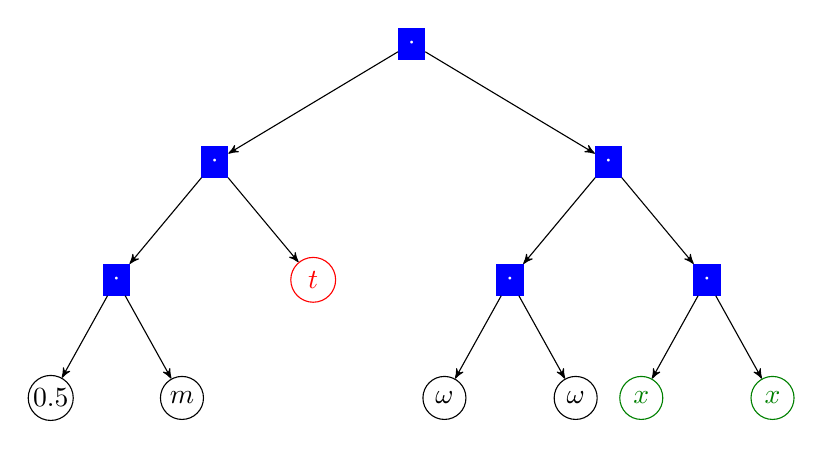
\begin{tikzpicture}[->,>=stealth',level/.style={sibling distance = 5cm/#1,
    level distance = 1.5cm}]
    \node [oprnode] {$\cdot$}
      child{ node [oprnode] {$\cdot$}
        child{ node [oprnode] {$\cdot$}
          child{ node [exprnode] {$0.5$}}
          child{ node [exprnode] {$m$}}
        }
        child{ node [varnode] {$t$}}
      }
      child{ node [oprnode] {$\cdot$}
        child{ node [oprnode] {$\cdot$}
          child{ node [exprnode] {$\omega$}}
          child{ node [exprnode] {$\omega$}}
        }
        child{ node [oprnode] {$\cdot$}
          child{ node [posnode] {$x$}}
          child{ node [posnode] {$x$}}
        }
      };
  \end{tikzpicture}
%\end{document}
